\documentclass[tikz, border=6pt]{standalone}
\usepackage[T1]{fontenc}
\usepackage{lmodern}
\usepackage{amsmath,amssymb,bm}
\usepackage{lmodern}
\usetikzlibrary{arrows.meta}
\definecolor{Ink}{HTML}{1F2937}
\tikzset{
  cd arrow/.style={line width=0.5pt, >={Computer Modern Rightarrow[length=3.2pt, width=5.6pt]}, ->, shorten <=2pt, shorten >=2pt},
  cd label/.style={font=\small, inner sep=2.5pt},
}
\begin{document}
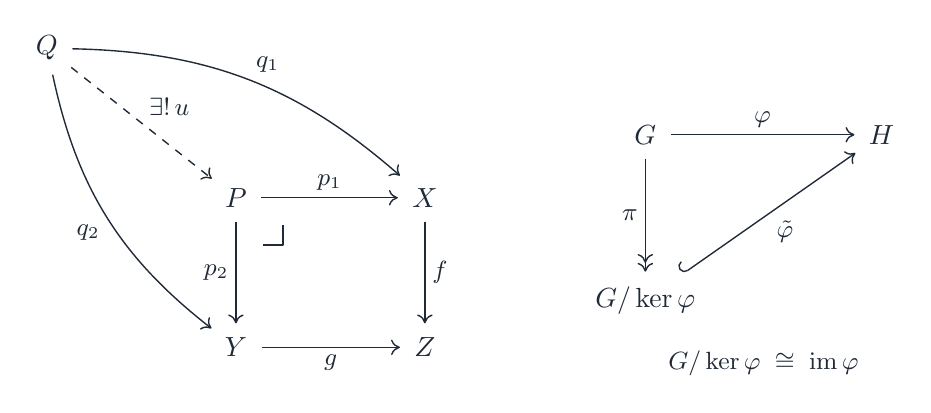
\begin{tikzpicture}[color=Ink, line width=0.5pt, >={Latex[length=5pt, width=3.6pt]}, line join=round]
  % commutative diagram pb
  \node[inner sep=3pt] (pb-0-0) at (0,0) {$Q$};
  \node[inner sep=3pt] (pb-1-1) at (2.4,-1.9) {$P$};
  \node[inner sep=3pt] (pb-1-2) at (4.8,-1.9) {$X$};
  \node[inner sep=3pt] (pb-2-1) at (2.4,-3.8) {$Y$};
  \node[inner sep=3pt] (pb-2-2) at (4.8,-3.8) {$Z$};
  \draw[cd arrow] (pb-1-1) -- node[cd label, auto, pos=0.5] {$p_1$} (pb-1-2);
  \draw[cd arrow] (pb-1-1) -- node[cd label, auto, swap, pos=0.5] {$p_2$} (pb-2-1);
  \draw[cd arrow] (pb-1-2) -- node[cd label, auto, pos=0.5] {$f$} (pb-2-2);
  \draw[cd arrow] (pb-2-1) -- node[cd label, auto, swap, pos=0.5] {$g$} (pb-2-2);
  \draw[cd arrow, dashed] (pb-0-0) -- node[cd label, auto, pos=0.5] {$\exists!\,u$} (pb-1-1);
  \draw[cd arrow] (pb-0-0) to[bend left=20] node[cd label, auto, pos=0.5] {$q_1$} (pb-1-2);
  \draw[cd arrow] (pb-0-0) to[bend right=20] node[cd label, auto, swap, pos=0.5] {$q_2$} (pb-2-1);
  \draw[line width=0.5pt] (2.75,-2.5) -- (3,-2.5) -- (3,-2.25);
  % commutative diagram iso
  \node[inner sep=3pt] (iso-0-0) at (7.6,-1.1) {$G$};
  \node[inner sep=3pt] (iso-0-1) at (10.6,-1.1) {$H$};
  \node[inner sep=3pt] (iso-1-0) at (7.6,-3.2) {$G/\ker\varphi$};
  \draw[cd arrow] (iso-0-0) -- node[cd label, auto, pos=0.5] {$\varphi$} (iso-0-1);
  \draw[cd arrow, ->>] (iso-0-0) -- node[cd label, auto, swap, pos=0.5] {$\pi$} (iso-1-0);
  \draw[cd arrow, {Hooks[right,length=2.2pt]}->] (iso-1-0) -- node[cd label, auto, swap, pos=0.5] {$\tilde\varphi$} (iso-0-1);
  \node[font=\small] at (9.1,-4) {$G/\ker\varphi \;\cong\; \operatorname{im}\varphi$};
\end{tikzpicture}
\end{document}
